\documentclass{article}
\usepackage[utf8]{inputenc}
\usepackage{amsmath}
\usepackage{amsfonts}
\usepackage{graphicx}
\usepackage{booktabs}
\usepackage{amssymb}
\usepackage{ragged2e}
\usepackage{geometry}
\usepackage{float}
\usepackage{longtable} 
\usepackage{verbatim} 
\usepackage{tabularx}
\usepackage[table]{xcolor}
\newcolumntype{C}{>{\centering\arraybackslash}X}
\usepackage{subcaption}

\usepackage{bm}
\usepackage{tikz}
\usetikzlibrary{
  arrows.meta,
  positioning,
  shapes.geometric,
  calc,
  fit,
  backgrounds,
  quotes, 
  decorations.pathreplacing 
}
\tikzset{
  every node/.style={inner sep=2pt}
}


\definecolor{inputGreen}{RGB}{225, 245, 238}
\definecolor{inputGreenBorder}{RGB}{15, 110, 86}
\definecolor{encoderGray}{RGB}{241, 239, 232}
\definecolor{encoderGrayBorder}{RGB}{95, 94, 90}
\definecolor{computeBlue}{RGB}{230, 241, 251}
\definecolor{computeBlueBorder}{RGB}{24, 95, 165}
\definecolor{stagePurple}{RGB}{238, 237, 254}
\definecolor{stagePurpleBorder}{RGB}{83, 74, 183}
\definecolor{projOrange}{RGB}{250, 236, 231}
\definecolor{projOrangeBorder}{RGB}{153, 60, 29}
\definecolor{codebookYellow}{RGB}{250, 238, 218}
\definecolor{codebookYellowBorder}{RGB}{133, 79, 11}
\definecolor{deadGreen}{RGB}{234, 243, 222}
\definecolor{deadGreenBorder}{RGB}{59, 109, 17}

\title{Beyond Reward Suppression: Reshaping Steganographic Communication Protocols in MARL via Dynamic Representational Circuit Breaking}
\author{Liu Hung Ming\thanks{PARRAWA AI} \\ {cyril.liu@gmail.com}}

\begin{document}

\maketitle 

\begin{abstract}
\end{abstract}

\section{Methods}
\subsection{Dataset and Experimental Design}\label{sec:dataset}
\begin{figure}[H]
  \centering
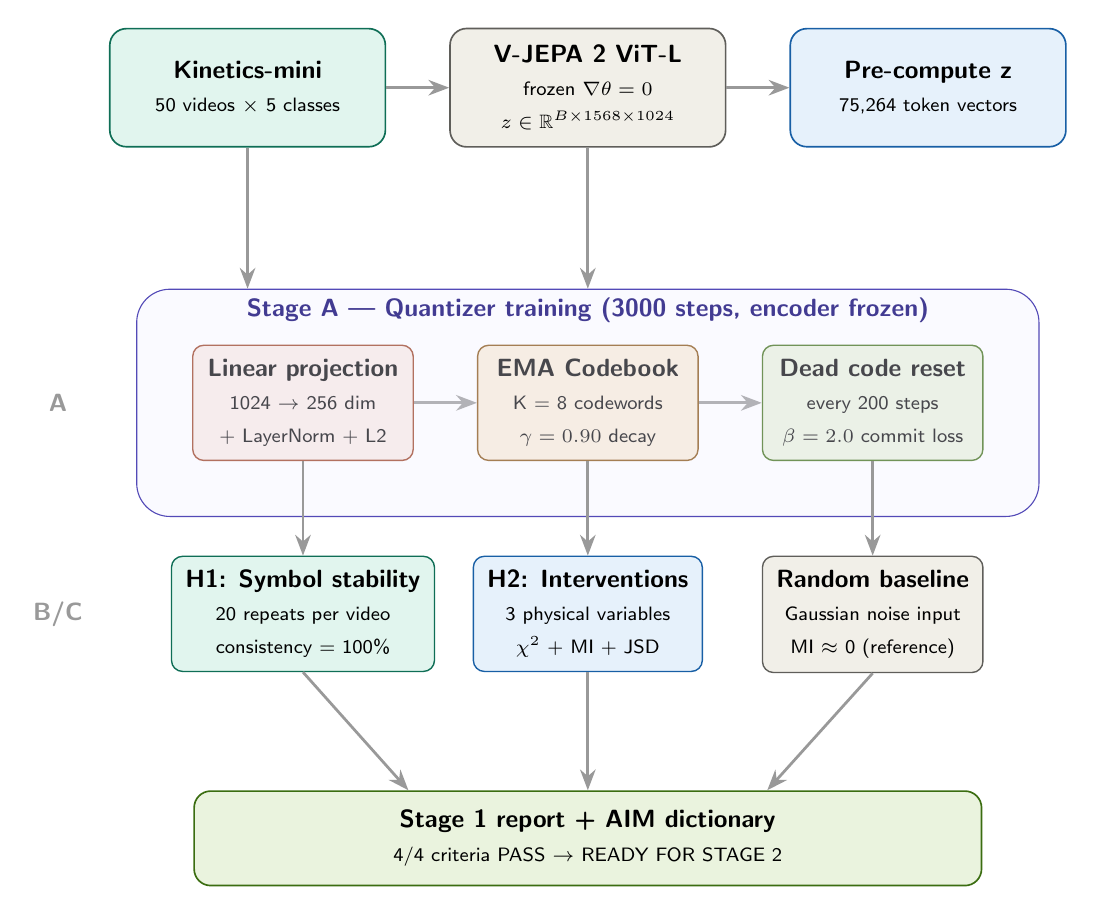
\begin{tikzpicture}[
    font=\sffamily,
    node distance=1.2cm and 0.8cm,
    box/.style={rectangle, draw, rounded corners=6pt, inner sep=6pt, align=center, line width=0.6pt, minimum height=1.5cm},
    subbox/.style={rectangle, draw, rounded corners=4pt, inner sep=5pt, align=center, line width=0.5pt, minimum height=1.3cm, minimum width=2.8cm},
    arrow/.style={-{Stealth[scale=1.0]}, draw=gray!80, line width=1pt}
]

 
    \node[box, fill=encoderGray, draw=encoderGrayBorder, minimum width=3.5cm] (encoder) {
        \textbf{\small V-JEPA 2 ViT-L} \\ \scriptsize frozen $\nabla\theta = 0$ \\ \scriptsize $z \in \mathbb{R}^{B \times 1568 \times 1024}$
    };
    
    \node[box, fill=inputGreen, draw=inputGreenBorder, left=of encoder, minimum width=3.5cm] (input) {
        \textbf{\small Kinetics-mini} \\ \scriptsize 50 videos $\times$ 5 classes
    };

    \node[box, fill=computeBlue, draw=computeBlueBorder, right=of encoder, minimum width=3.5cm] (compute) {
        \textbf{\small Pre-compute z} \\ \scriptsize 75,264 token vectors
    };
        
        

    \draw[arrow] (input) -- (encoder);
    \draw[arrow] (encoder) -- (compute);


    \node[subbox, fill=codebookYellow, draw=codebookYellowBorder, below=2.5cm of encoder] (codebook) {
        \textbf{\small EMA Codebook} \\ \scriptsize K = 8 codewords \\ \scriptsize $\gamma = 0.90$ decay
    };

    \node[subbox, fill=projOrange, draw=projOrangeBorder, left=of codebook] (proj) {
        \textbf{\small Linear projection} \\ \scriptsize 1024 $\to$ 256 dim \\ \scriptsize + LayerNorm + L2
    };

    \node[subbox, fill=deadGreen, draw=deadGreenBorder, right=of codebook] (dead) {
        \textbf{\small Dead code reset} \\ \scriptsize every 200 steps \\ \scriptsize $\beta = 2.0$ commit loss
    };

    \draw[arrow] (proj) -- (codebook);
    \draw[arrow] (codebook) -- (dead);


    \node[fit=(proj) (dead), rectangle, draw=stagePurpleBorder, fill=stagePurple, fill opacity=0.3, rounded corners=12pt, inner sep=20pt ] (stageA) {};
    \node[anchor=north, text=stagePurpleBorder!80!black, yshift=-1pt] at (stageA.north) {\textbf{\small Stage A --- Quantizer training (3000 steps, encoder frozen)}};
    
   
    \node[left=0.8cm of stageA.west, text=gray!80] (labelA) {\textbf{\small A}};

  
    \draw[arrow] (input.south) -- (input.south |- stageA.north);
    \draw[arrow] (encoder.south) -- (encoder.south |- stageA.north);

  
    \node[subbox, fill=inputGreen, draw=inputGreenBorder, below=1.2cm of proj] (h1) {
        \textbf{\small H1: Symbol stability} \\ \scriptsize 20 repeats per video \\ \scriptsize consistency = 100\%
    };

    \node[subbox, fill=computeBlue, draw=computeBlueBorder, below=1.2cm of codebook] (h2) {
        \textbf{\small H2: Interventions} \\ \scriptsize 3 physical variables \\ \scriptsize $\chi^2$ + MI + JSD
    };

    \node[subbox, fill=encoderGray, draw=encoderGrayBorder, below=1.2cm of dead] (baseline) {
        \textbf{\small Random baseline} \\ \scriptsize Gaussian noise input \\ \scriptsize MI $\approx$ 0 (reference)
    };
    

    \node[at=(h1 -| labelA), text=gray!80] {\textbf{\small B/C}};

  
    \draw[arrow] (proj.south) -- (h1.north);
    \draw[arrow] (codebook.south) -- (h2.north);
    \draw[arrow] (dead.south) -- (baseline.north);


    \node[box, fill=deadGreen, draw=deadGreenBorder, below=1.5cm of h2, minimum width=10cm, minimum height=1.2cm] (output) {
        \textbf{\small Stage 1 report + AIM dictionary} \\ \scriptsize 4/4 criteria PASS $\rightarrow$ READY FOR STAGE 2
    };


    \draw[arrow] (h1.south) -- (output.165);
    \draw[arrow] (h2.south) -- (output.north);
    \draw[arrow] (baseline.south) -- (output.15);

\end{tikzpicture}
\caption{Stage~1 pipeline overview.
         \textit{Top row} (A): The input pipeline feeds 50 Kinetics-mini
         videos through the frozen V-JEPA~2 ViT-L encoder
         ($\nabla\theta = 0$), producing $B \times 1568 \times 1024$
         latent token vectors that are precomputed once and cached.
         \textit{Middle row} (A): The Stage~A quantizer trains for 3,000
         steps on the precomputed vectors using a linear projection layer
         ($1024 \to 256$ dimensions, followed by LayerNorm and L2
         normalization), an EMA-updated codebook ($K = 8$,
         $\gamma = 0.90$), and a dead-code reset mechanism
         ($\beta = 2.0$ commitment loss); the V-JEPA~2 encoder weights
         remain fully frozen throughout.
         \textit{Bottom row} (B/C): After training, the pipeline is
         evaluated on two diagnostic criteria: H1 symbol stability
         (20 repeated forward passes per video; consistency $= 100\%$)
         and H2 intervention experiments (three physical-variable pairs
         assessed via $\chi^2$, MI, and JSD), with a Gaussian-noise
         random baseline confirming MI $\approx 0$ for unstructured
         inputs.  All four pass criteria are satisfied, producing the
         Stage~1 report and AIM dictionary that certify readiness for
         Stage~2.}
  \label{fig:pipeline_overview}
\end{figure}

Figure~\ref{fig:pipeline_overview} provides an overview of the
complete Stage~1 pipeline, from data ingestion through quantizer
training to diagnostic evaluation.

\paragraph{Dataset.}
We use the validation split of the Kinetics-mini dataset, selecting five action
categories: \textit{archery}, \textit{bowling}, \textit{flying\_kite},
\textit{high\_jump}, and \textit{marching}, with at most 10 videos per category.
Of these, 48 videos ultimately entered training (see Section~\ref{sec:frozen_encoder} for details).
Each video is sampled at $T = 16$ frames at $224\times224$ resolution, processed
through V-JEPA~2's official processor with center cropping and ImageNet
normalization before being passed to the encoder.

\paragraph{Rationale for the Intervention Design.}
The central question of Stage~1 is whether AIM's symbolization mechanism can
read structured information from V-JEPA~2's frozen latent space.  To investigate
this, we design controlled intervention experiments: all other conditions are
held fixed while a single physical dimension is varied, and we observe whether
the AIM symbol distribution changes in a statistically significant manner.

Kinetics-mini is an action-classification dataset whose labels denote action
categories rather than physical attributes.  It is therefore impossible to
directly manipulate a single physical variable (e.g., holding scene, subject,
and action constant while varying only grasp angle).  Instead, we adopt a
\textbf{category-proxy} strategy: we select pairs of action categories that
exhibit large natural differences along one target physical dimension while
minimizing differences along other major visual dimensions, using inter-category
contrast as a proxy for physical-variable contrast.

The validity of this strategy rests on the following premise.  V-JEPA~2 is
pretrained to predict masked spatiotemporal regions in latent space, so its
encoder must compress video into structured representations that support
spatiotemporal prediction.  Such representations inevitably encode physical
attributes such as object shape, pose, and motion pattern.  When two action
categories differ substantially along one physical dimension, that difference
should leave a measurable directional shift in latent space.  Stage~1 tests
whether this shift is sufficiently pronounced to be captured by AIM's discrete
symbolization mechanism.  Kinetics-mini serves as a publicly reproducible
benchmark providing a verifiable starting point.

Two practical reasons motivate the use of an existing video dataset rather than
purpose-built controlled footage.  First, the goal of this stage is
\emph{diagnostic}: to verify architectural compatibility between AIM and
V-JEPA~2, not to precisely quantify the encoding strength of specific physical
variables.  Category proxies are sufficient for the statistical-significance
tests that serve this purpose.  Second, acquiring video data with fine-grained
control over individual physical variables requires dedicated data-collection
infrastructure that exceeds the resource scope of Stage~1.

\paragraph{Category Pair Selection.}
The five categories are grouped into three contrastive pairs, each targeting one
physical dimension.  Pairs were chosen to maximize inter-category differences
along the target dimension while minimizing differences along other salient
visual features (e.g., scene type, number of persons, range of motion), thereby
reducing confounding variables.

\begin{itemize}
  \item \textbf{Grasp angle.}
    \textit{Archery} (drawing a bow: three-finger pinch grip on the string,
    arm extended into a static release posture with shoulder rotation)
    vs.\ \textit{bowling} (single-hand grip through finger holes, dynamic
    forward-swing throw).
    Both involve a single person, a hand-held object, and upper-limb-dominated
    motion; the primary differences are grip morphology and the direction of
    arm force application.  We note that scene environment (outdoor archery
    range vs.\ indoor bowling lane) and background color also differ---an
    unavoidable confound of the category-proxy strategy.

  \item \textbf{Object geometry.}
    \textit{Flying\_kite} (an elongated linear object controlled indirectly via
    string) vs.\ \textit{high\_jump} (no manipulated object; the subject's body
    executes an arching leap).
    The two conditions differ markedly in the geometry of the primary object and
    in the spatial relationship between the human body and that object.

  \item \textbf{Motion speed / temporal structure.}
    \textit{Marching} (periodic, regular gait with a $\approx$2\,Hz repetitive
    temporal structure) vs.\ \textit{archery} (near-static loading followed by a
    single rapid release; aperiodic temporal structure).
    Because V-JEPA~2's pretraining objective directly involves temporal
    prediction, we expect it to be most sensitive to temporal-structure
    differences---a prediction that is consistent with the experimental results,
    in which the motion-speed intervention yields the highest MI and JSD of the
    three pairs (Section~\ref{sec:h2_results}).
\end{itemize}

\paragraph{Reuse of Archery.}
\textit{Archery} appears in both the grasp-angle pair (contrasted with bowling)
and the motion-speed pair (contrasted with marching).  This is a design
compromise imposed by the limited dataset scale, but it simultaneously provides
an additional validation opportunity: if AIM's symbol system captures stable
latent features of the action category rather than incidental statistical
artifacts introduced by the intervention framework, then \textit{archery} should
produce consistent symbol distributions across the two independent interventions.
The experimental results confirm this (Section~\ref{sec:h2_results}).

\paragraph{Limitations of the Category-Proxy Strategy.}
The fundamental limitation of this approach is that the symbol-distribution
differences we observe reflect the overall differences between the selected
action categories in V-JEPA~2's latent space, not the isolated effect of the
target physical variable.  For the grasp-angle intervention, for instance, the
latent-space distance between \textit{archery} and \textit{bowling} subsumes
contributions from grasp angle, scene environment, object material, and other
factors that the experimental design cannot disentangle.  The correct
characterization of our results is therefore: \emph{AIM symbols have
statistically significant discriminative power for action-category pairs whose
primary difference lies along a specified physical dimension}---not that AIM
symbols directly encode the target physical variable.  Ideal follow-up
validation should employ carefully controlled synthetic or robot-manipulation
videos that isolate the target variable while holding all other visual factors
constant; this is deferred to Stage~3 or future work.

\subsection{Frozen V-JEPA~2 Encoder and Latent Space Precomputation}\label{sec:frozen_encoder}



\paragraph{Scientific Necessity of the Freezing Strategy.}
The core scientific question of this stage is whether AIM's symbolization
mechanism can read knowledge already acquired by V-JEPA~2.  If the encoder were
left unfrozen, two confounds would be introduced: (1) the encoder could
actively adapt its output distribution in response to the quantizer, and
(2) the quantizer could acquire separability through encoder gradients that
would not otherwise exist.  Freezing the encoder ensures that, for any input
$\mathbf{x}$, the mapping $E_\phi(\mathbf{x})$ is constant and all parameter
gradients are fully blocked:
%
\begin{equation}
  \forall\,\theta \in \Phi:\quad
  \frac{\partial \mathcal{L}}{\partial \theta} = 0,
  \qquad E_\phi(\cdot)\big|_{\text{eval}}.
\end{equation}
%
Freezing also yields a practical benefit: because a frozen encoder produces
identical outputs for identical inputs, all latent vectors $\mathbf{z}$ can be
precomputed once and reused throughout training, eliminating the need to
re-execute an encoder forward pass at every training step.

\paragraph{Preliminary Latent Space Diagnosis.}
Prior to designing the quantizer, we executed
 to characterize the numerical
properties of V-JEPA~2's output distribution across 5
representative videos.  This diagnostic revealed the key
challenge: the per-token L2 norm of $97.70 \pm 0.81$ is
exceptionally large and highly uniform (coefficient of
variation $< 0.6\%$), meaning that all latent vectors are
nearly equidistant from any randomly initialized codebook
entry.  Direct quantization without normalization would
therefore cause immediate codebook collapse, a finding that
directly motivated the projection-plus-normalization pipeline
described in Section~\ref{sec:quantizer}.
\paragraph{Token Structure of V-JEPA~2 ViT-L.}
V-JEPA~2 uses tubelet embedding with temporal patch size $t_p = 2$ and spatial
patch size $p = 16$.  For $T = 16$ input frames the number of output tokens is
%
\begin{equation}
  N_{\text{tokens}}
  = \frac{T}{t_p} \times \left(\frac{H}{p}\right)^2
  = \frac{16}{2} \times \left(\frac{224}{16}\right)^2
  = 8 \times 196
  = 1{,}568.
\end{equation}
%
Each tubelet token spans 2 frames in time and a $16\times16$ pixel patch in
space.  With embedding dimension $D = 1{,}024$, the encoder output for a batch
of $B$ videos is
%
\begin{equation}
  \mathbf{Z} = E_\phi(\mathcal{V}) \in \mathbb{R}^{B \times 1568 \times 1024}.
\end{equation}
%
Measurements on 5 representative videos show that the L2 norm of the latent
vectors satisfies $\|\mathbf{z}\|_2 = 97.70 \pm 0.81$ (range
$[96.26,\,98.58]$), a coefficient of variation below $0.6\%$.  This high
consistency is a systematic property of V-JEPA~2 rather than a coincidence;
however, the absolute magnitude is so large that direct quantization inevitably
distorts distance computations---all vectors are nearly equidistant from any
codebook entry.

\paragraph{Spatial Token Retention (Discarding Temporal Pooling).}
An earlier experimental version applied temporal pooling:
%
\begin{equation}
  \mathbf{z}_{\text{frame},t}
  = \frac{1}{196}\sum_{k=1}^{196}\mathbf{Z}_{t,k}
  \in \mathbb{R}^{1024},
\end{equation}
%
averaging the 196 spatial tokens for each time step.  This operation reduced
codebook utilization to only 5\% and caused the grasp-angle intervention to
fail statistical significance ($p = 0.357$).  The root cause is that mean
pooling erases spatial local semantic differences: the distributional contrast
between hand-pose tokens and background tokens is diluted into a single
per-frame average.

The final design retains all spatial tokens:
%
\begin{equation}
  \mathbf{z}_{\text{all}}
  = \operatorname{reshape}\!\bigl(\mathbf{Z},\;
    [B \cdot 1568,\; 1024]\bigr).
\end{equation}
%
The validity of this design presupposes that V-JEPA~2's latent vectors are
semantically diverse across the spatial dimension.  The 1,568 tokens are not
homogeneous: each corresponds to a distinct $16\times16$ pixel patch and carries
independent local semantics (hand pose, background texture, target-object shape,
etc.).  Temporal pooling actively destroys this diversity; retaining spatial
tokens allows the quantizer to learn patch-level semantic clusters directly.

In practice, the DataLoader scanned 50 videos with \texttt{drop\_last=True} and
batch size 16, so precomputation used
$\lfloor 50/16\rfloor \times 16 = 48$ videos, yielding
$48 \times 1{,}568 = 75{,}264$ token vectors---a 94-fold increase over the
800 vectors produced by temporal pooling.

Retaining raw spatial tokens allows different codebook entries to correspond to
local concepts such as ``hand motion,'' ``static background,'' and ``dynamic
foreground,'' rather than uninterpretable global averages.  This explains the
improvement in codebook utilization from 5\% (temporal pooling) to 62.5\%
(spatial tokens): the former provides training samples that are too homogeneous,
whereas the latter supplies the semantic diversity that codebook learning
requires.

\subsection{Stage~1 Lightweight AIM Quantizer (Stage~A)}\label{sec:quantizer}

\paragraph{Architecture Overview.}
The quantizer is a single-layer vector quantization (VQ) module; the only
trainable components are the projection layer $\mathbf{W}_p$ and the
EMA-updated codebook $\mathcal{C}$.  The single-layer design is deliberate:
the goal of Stage~1 is diagnostic---to verify architectural compatibility
between AIM and V-JEPA~2---and a single-layer VQ already provides sufficient
signal for the H2 statistical tests.  Residual quantization is deferred to
Stage~2.
\paragraph{Implementation Note.}
The Stage~1 quantizer described in this section is implemented as the
\texttt{Stage1AIMQuantizer} class.
A separate multi-level residual VQ architecture (\texttt{AIMQuantizerForVJEPA}
, $L = 3$ levels with codebook sizes
$\{64, 128, 256\}$) is reserved for Stage~2 and is not used in any
experiment reported here.  All hyperparameters reported in this section
(Table~\ref{tab:ablation}: $\gamma = 0.90$, $\beta = 2.0$, $K = 8$)
were passed as command-line arguments to,
overriding the class-level defaults retained for backward compatibility.
Stage 1 results are derived solely from the primary diagnostic framework. The Stage 2-ready architecture lacks the essential normalization pipeline; as such, it is incompatible with the frozen latent space under the current diagnostic constraints and would lead to a total loss of codebook utilization if applied here.

\paragraph{Projection Health Verification.}
Before committing to the full training run, we verified the
projection layer's behavior,
which confirmed that: (1) LayerNorm successfully stabilizes the
projected norm to $\sqrt{d_{\text{proj}}} = 16.00$ (std $= 1.0005$);
(2) subsequent L2 normalization correctly maps all vectors onto the
unit hypersphere; and (3) cosine similarity between projected vectors
from different inputs is $\approx 0.03$, confirming that the vectors
are well-separated and not collapsing to a single direction.  These checks established the parameter configuration ($d_{\text{proj}} = 256$,
LayerNorm before L2 normalization) before the hyperparameter search for
$\gamma$ and $\beta$ described in the ablation study below.


 
\paragraph{Step~1: Projection and Normalization.}
Because the L2 norm of V-JEPA~2 ViT-L outputs satisfies
$\|\mathbf{z}\|_2 = 97.70 \pm 0.81$ (mean $\pm$ std across 5 videos,
range $[96.26,\,98.58]$), direct quantization would cause codebook
collapse---all vectors are nearly equidistant from any codebook entry.
The system therefore applies a linear projection followed by
LayerNorm:
%
\begin{equation}
  \mathbf{z}_{\text{proj}}
  = \operatorname{LayerNorm}(\mathbf{W}_p\,\mathbf{z} + \mathbf{b}_p),
  \qquad \mathbf{W}_p \in \mathbb{R}^{256 \times 1024}.
\end{equation}
%


LayerNorm standardizes each projected dimension (per-dimension mean $\to 0$,
std $\to 1$), stabilizing the overall L2 norm from the raw value of
$\approx\!97.7$ to $\sqrt{d_{\text{proj}}} = \sqrt{256} = 16$ (empirically
verified: post-LayerNorm norm $= 16.00$, std $= 1.0005$).  Note that LayerNorm
and L2 normalization play distinct roles: LayerNorm compresses the per-dimension
distribution but leaves the overall norm at 16, while the subsequent L2
normalization projects vectors onto the unit hypersphere.

All projected vectors are then L2-normalized onto the unit hypersphere:
%
\begin{equation}
  \hat{\mathbf{z}}
  = \frac{\mathbf{z}_{\text{proj}}}{\|\mathbf{z}_{\text{proj}}\|_2}
  \in \mathbb{S}^{255}.
\end{equation}
%
On the unit hypersphere, Euclidean distance and cosine similarity are
equivalent:
%
\begin{equation}
  \|\hat{\mathbf{z}}^{(i)} - \mathbf{c}_k\|_2^2
  = 2\bigl(1 - \hat{\mathbf{z}}^{(i)\top}\mathbf{c}_k\bigr).
\end{equation}
%
Codebook competition therefore depends solely on directional differences,
eliminating any influence of vector magnitude.  Empirical verification confirms
that the cosine similarity between projected vectors from different videos is
$0.03 \approx 0$, indicating that vectors are highly separable on the
hypersphere.

\paragraph{Step~2: Nearest-Neighbor Assignment (VQ).}
For codebook $\mathcal{C} = \{\mathbf{c}_1, \ldots, \mathbf{c}_K\}$ with
$K = 8$, each projected vector is assigned to its nearest entry:
%
\begin{equation}
  s^{(i)}
  = \arg\min_{k}\,\|\hat{\mathbf{z}}^{(i)} - \mathbf{c}_k\|_2^2
  = \arg\max_{k}\;\hat{\mathbf{z}}^{(i)\top}\mathbf{c}_k.
\end{equation}
%
The argmin-distance formulation is equivalent to argmax inner product and to
cosine-similarity search, enabling efficient batched computation.

\paragraph{Step~3: Straight-Through Estimator.}
Because the argmin operation is non-differentiable, we use the
straight-through estimator (STE)~\cite{bengio2013estimating} to route
gradients past the argmin directly to the projection layer:
%
\begin{equation}
  \mathbf{z}_q^{(i)}
  = \hat{\mathbf{z}}^{(i)}
    + \operatorname{sg}\!\bigl(\mathbf{c}_{s^{(i)}} - \hat{\mathbf{z}}^{(i)}\bigr),
\end{equation}
%
where $\operatorname{sg}(\cdot)$ denotes the stop-gradient operator.
In the forward pass $\mathbf{z}_q$ equals the selected codebook vector; in the
backward pass gradients flow directly through $\hat{\mathbf{z}}$ to the
projection layer $\mathbf{W}_p$.

\paragraph{Step~4: Commitment Loss.}
A commitment loss penalizes deviation of the projected output from the assigned
codebook entry, preventing drift in the projection layer:
%
\begin{equation}
  \mathcal{L}_{\text{commit}}
  = \beta \cdot
    \bigl\|\operatorname{sg}(\mathbf{c}_{s^{(i)}})
           - \hat{\mathbf{z}}^{(i)}\bigr\|_2^2,
  \qquad \beta = 2.0.
\end{equation}
%
The value $\beta = 2.0$ is substantially larger than the standard VQ-VAE value
of $0.25$~\cite{oord2017neural}; it was selected via the hyperparameter search
reported in Table~\ref{tab:ablation}.

\begin{table}[H]
\centering
\caption{Ablation of EMA decay rate and commitment loss coefficient.}
\label{tab:ablation}
\begin{tabular}{ccc}
\toprule
$\gamma$ (EMA decay) & $\beta$ (commitment) & Outcome \\
\midrule
0.99 & 0.25 & Codebook collapse; active ratio $< 5\%$ \\
0.95 & 1.0  & Collapse; perplexity continuously decreasing \\
0.90 & 2.0  & Stabilized; active ratio $= 62.5\%$; all criteria passed \\
\bottomrule
\end{tabular}
\end{table}

\paragraph{Step~5: EMA Codebook Update.}
Codebook vectors are not updated via gradients; instead, exponential moving
averages (EMA) with decay rate $\gamma = 0.90$ are used:
%
\begin{align}
  N_k^{(t)}
  &= \gamma\,N_k^{(t-1)}
   + (1-\gamma)\sum_{i=1}^{B}\mathbf{1}\bigl[s^{(i)}=k\bigr], \\[4pt]
  \mathbf{M}_k^{(t)}
  &= \gamma\,\mathbf{M}_k^{(t-1)}
   + (1-\gamma)\sum_{i=1}^{B}\mathbf{1}\bigl[s^{(i)}=k\bigr]
     \cdot\hat{\mathbf{z}}^{(i)}, \\[4pt]
  \mathbf{c}_k^{(t)}
  &= \frac{\mathbf{M}_k^{(t)}/\bigl(N_k^{(t)}+\epsilon\bigr)}
          {\bigl\|\mathbf{M}_k^{(t)}/\bigl(N_k^{(t)}+\epsilon\bigr)\bigr\|_2}.
\end{align}
%
Here $N_k$ tracks the hit frequency of each codebook entry and $\mathbf{M}_k$
accumulates the weighted sum of all assigned vectors; their ratio gives the
weighted mean position of the entry, which is then L2-normalized to keep all
codebook vectors on the unit hypersphere.

With $\gamma = 0.90$, the effective memory half-life of the EMA update is
%
\begin{equation}
  t_{1/2} = \frac{\ln 2}{\ln(1/\gamma)} \approx 6.6\ \text{steps},
\end{equation}
%
compared with $\approx\!69$ steps at the standard value $\gamma = 0.99$.  This
aggressive setting is necessary: the high compactness of V-JEPA~2's frozen
latent space causes the initial codebook to be easily dominated by a single
cluster, and a shorter memory half-life allows codebook entries to disperse
rapidly into different feature subspaces during early training.  The failure
case at $\gamma = 0.99$ in Table~\ref{tab:ablation} directly validates this
reasoning.

\paragraph{Step~6: Dead-Code Reset.}
Every 200 steps, entries whose usage fraction falls below $\tau/K$
($\tau = 0.01$) are declared dead and replaced by the highest-variance vector
in the current batch:
%
\begin{equation}
  \text{dead}_k
  = \frac{N_k}{\sum_j N_j} < \frac{0.01}{K},
  \qquad
  \mathbf{c}_k \leftarrow \hat{\mathbf{z}}^{(i^*)},
  \quad
  i^* = \arg\max_{i}\,\operatorname{Var}(\hat{\mathbf{z}}^{(i)}).
\end{equation}

\paragraph{Codebook Health Monitoring.}
Codebook utilization uniformity is measured by perplexity:
%
\begin{equation}
  \text{Perplexity}
  = \exp\!\left(-\sum_{k=1}^{K} p_k \ln p_k\right),
  \quad p_k = \frac{N_k}{\sum_j N_j}.
\end{equation}
%
The maximum value is $K = 8$ (perfectly uniform distribution); the health
threshold is set at $0.4 \times K = 3.2$.  At the end of training, $\text{Perplexity} = 4.635$
(as recorded in \texttt{stage1\_report.json} under
\texttt{final\_perplexity}; a slightly different value of $4.707$
appears under \texttt{codebook\_active} due to a separate
evaluation pass after training completion), corresponding to a utilization uniformity of
$4.635/8 = 57.9\%$, well above the threshold.


\paragraph{K-means Initialization.}
To avoid immediate collapse from random initialization, the codebook is
initialized with real latent vectors: $K$ post-projection vectors are sampled
uniformly at random from the 75,264 precomputed tokens and used as initial
codebook entries, with EMA statistics initialized as $\mathbf{M}_k = \mathbf{c}_k$
and $N_k = 1$ to prevent division by zero.

\paragraph{Optimizer.}
Only the projection layer is updated by gradients, using Adam with learning rate
$\eta_0 = 10^{-3}$ and cosine annealing to $\eta_{\min} = 10^{-4}$:
%
\begin{equation}
  \eta_t
  = \eta_{\min}
  + \frac{1}{2}(\eta_0 - \eta_{\min})
    \left(1 + \cos\frac{\pi t}{T_{\max}}\right).
\end{equation}
%
Training runs for 3,000 steps with a batch size of 64 token vectors sampled
randomly from the 75,264 precomputed vectors.  V-JEPA~2 encoder weights remain
fully frozen throughout.

\subsection{H1: Symbol Stability Test}\label{sec:h1_stability}

\paragraph{Test Design.}
After training, the quantizer is switched to evaluation mode
(\texttt{quantizer.eval()}), at which point the codebook ceases to update,
dropout is disabled, and batch normalization statistics are fixed, making the
entire forward pass a deterministic function.  The same video is passed through
the pipeline $M = 20$ independent times, and the representative symbol for each
run is computed as the mode over all spatial tokens:
%
\begin{equation}
  s_{\text{video}}^{(m)}
  = \operatorname{mode}\bigl\{s_j^{(m)} : j = 1, \ldots, N_{\text{tokens}}\bigr\},
  \quad m = 1, \ldots, 20.
\end{equation}
%
Stability is defined as the fraction of the 20 runs in which the mode symbol
agrees with the first run:
%
\begin{equation}
  \text{Stability}_{\text{video}}
  = \frac{1}{M}\sum_{m=1}^{M}
    \mathbf{1}\!\left[s_{\text{video}}^{(m)} = s_{\text{video}}^{(1)}\right].
\end{equation}
%
The overall H1 score is the mean stability across all test videos,
$\bar{\rho} = \frac{1}{|\mathcal{V}_{\text{stab}}|}\sum_{v}\text{Stability}_v$,
with passing criterion $\bar{\rho} > 0.95$.

\paragraph{Scientific Significance and Design Limitations.}
It is important to note that, under the spatial-token-plus-mode design, $H1 =
1.000$ is a mathematical certainty in eval mode with a frozen encoder: the
encoder is a deterministic function (no dropout), and the argmin quantization
step is likewise deterministic, so identical inputs must produce identical mode
symbols.  Compared with the original temporal-pooling design---in which each
frame was quantized independently and the resulting 16-symbol sequence could be
destabilized by data augmentation or model stochasticity---the spatial-token
design narrows the scope of H1 from \emph{semantic stability of the symbol
sequence} to \emph{pipeline determinism verification}.

Accordingly, the scientific role of H1 in this experiment is that of a
necessary precondition check rather than independent evidence of semantic
stability.  It confirms that the entire pipeline (random cropping disabled in
the processor: \texttt{do\_random\_crop=False}; all stochastic layers fixed in
the encoder: \texttt{encoder.eval()}) retains no residual randomness, thereby
guaranteeing that any symbol-distribution differences observed in the H2
intervention experiments arise solely from differences in the input conditions
and not from internal pipeline noise.  The statistical evidence that genuinely
supports symbol validity comes from the chi-squared tests, mutual information,
and Jensen--Shannon divergence reported in the H2 intervention experiments
(Section~\ref{sec:h2_results}).

\subsection{H2: Statistical Framework for Intervention Experiments}

\paragraph{Symbol Distribution Collection.}
For each condition $c \in \{c_1, \ldots, c_C\}$, we collect $n_c$ video
samples.  The representative symbol for each video is computed as the mode over
all spatial tokens:
%
\begin{equation}
  s_{\text{video}}
  = \operatorname{mode}\bigl\{s_j : j = 1, \ldots, 1568\bigr\}.
\end{equation}
%
These per-video symbols are aggregated into an observed frequency matrix
$O \in \mathbb{Z}^{C \times K}$, where $O_{c,k}$ denotes the number of times
symbol $k$ appears under condition $c$.

\paragraph{Chi-Squared Independence Test (H2a).}
The null hypothesis $H_0$ states that the symbol distribution is independent
of the physical condition.  The test statistic is
%
\begin{equation}
  \chi^2
  = \sum_{c=1}^{C}\sum_{k=1}^{K}
    \frac{(O_{c,k} - E_{c,k})^2}{E_{c,k}},
  \qquad
  E_{c,k} = \frac{R_c \cdot C_k}{N},
\end{equation}
%
with degrees of freedom $\mathrm{df} = (C-1)(K-1) = 7$ (since $C = 2$ and
$K = 8$).  $H_0$ is rejected when $p < 0.01$.

\paragraph{Mutual Information (H2b).}
The mutual information between the symbol $S$ and the physical condition label
$L$ is estimated using a Laplace-smoothed plug-in estimator:
%
\begin{equation}
  I(S;\,L)
  = \sum_{s}\sum_{l}
    \hat{p}(s,l)\log\frac{\hat{p}(s,l)}{\hat{p}(s)\,\hat{p}(l)}.
\end{equation}

\paragraph{MI Ratio (H2c).}
A random baseline MI is computed by passing Gaussian noise inputs through the
full pipeline.  The MI ratio for each experimental condition is then defined as
%
\begin{equation}
  \text{MI Ratio}
  = \frac{I(S;\,L)_{\text{experiment}}}
         {I(S;\,L)_{\text{random}} + \epsilon},
  \qquad \epsilon = 10^{-8}.
\end{equation}
%
We note that this baseline differs from the permutation test standard in the
causal-inference literature, which constructs an empirical null distribution by
randomly shuffling condition labels.  The Gaussian-noise baseline answers the
question ``does the codebook exhibit a prior preference for unstructured
inputs?'' (baseline MI $< 10^{-7}$), whereas a permutation test would answer
``how likely is the observed MI to arise by chance from the condition grouping
alone?''---two fundamentally distinct questions.  Given that the chi-squared
$p$-values are far below any reasonable significance threshold, this design
choice does not affect the qualitative conclusions; however, future work should
incorporate permutation testing to strengthen methodological rigor.

\paragraph{Pairwise Jensen--Shannon Divergence (H2d).}
The distributional distance between two conditions is quantified by the
Jensen--Shannon divergence (JSD):
%
\begin{equation}
  \mathrm{JSD}(P_{c_i} \| P_{c_j})
  = \frac{1}{2}D_{\mathrm{KL}}(P_{c_i} \| M)
  + \frac{1}{2}D_{\mathrm{KL}}(P_{c_j} \| M),
  \qquad
  M = \frac{P_{c_i} + P_{c_j}}{2},
\end{equation}
%
where $\mathrm{JSD} \in [0,\,1]$, with larger values indicating greater
divergence between the symbol distributions of the two conditions.
\section{Experiments and Results} 
\subsection{Quantizer Training Convergence (Stage~A)}

Figure~\ref{fig:stage_a_training} shows the commitment loss and codebook
perplexity curves over the full 3,000-step training run.

Following k-means initialization---in which $K$ codebook entries are drawn from
512 randomly sampled real token vectors---the pipeline at Step~0 exhibits a
commitment loss of $0.0086$, a perplexity of $6.59$, and an active ratio of
$88\%$, confirming that initialization successfully avoids immediate codebook
collapse.

The commitment loss decreases rapidly from $0.0086$ to below $0.0001$ within
the first 200 steps and remains stable thereafter.  Codebook perplexity
converges from the initial value of $6.59$ to a final value of $4.635$
(maximum possible $K = 8$; health threshold $0.4 \times K = 3.2$), yielding
a utilization uniformity of $\text{Perplexity}/K = 57.9\%$, well above the
$30\%$ passing criterion.  

Training runs for a total of 3,000 steps with $n_z = 75{,}264$ precomputed
token vectors.  The final active ratio---the fraction of codebook entries with
a non-zero usage counter---is $\mathbf{62.5\%}$ (5 out of $K = 8$ entries
actively used).  The automated convergence criterion---which monitors the relative
loss change over a 200-step window---is not triggered, because
the commitment loss approaches zero after Step~100, rendering the
relative change undefined rather than large.  The diagnostic log
therefore records \texttt{converged: false}, which reflects a
boundary condition in the stopping criterion implementation rather
than a failure to stabilize.  Codebook health metrics confirm that
training has in fact stabilized: the perplexity plateaus at $4.635$
and the active ratio remains constant at $62.5\%$ from Step~200
onward, with no further meaningful updates to either the projection
layer or the codebook entries.

\begin{figure}[H]
  \centering
\makebox[\textwidth][c]{%
    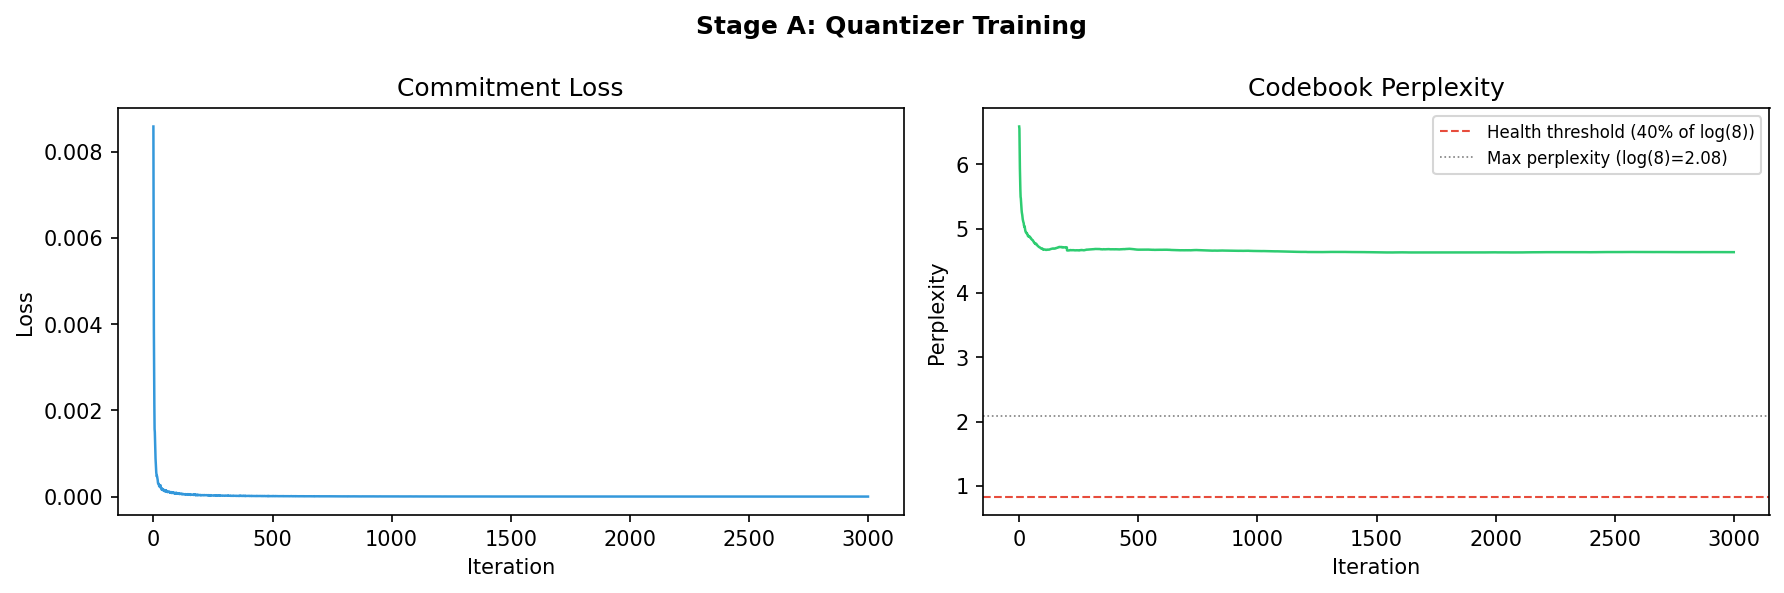
\includegraphics[width=1.3\linewidth]{stage_a_training.png}%
    }
  \caption{Stage~A quantizer training curves.
           \textit{Left}: commitment loss as a function of training iteration,
           showing rapid convergence within the first 200 steps.
           \textit{Right}: codebook perplexity trajectory; the red dashed line marks the health threshold
($0.4 \times K = 3.2$, corresponding to $40\%$ utilization uniformity),
and the grey dotted line marks the theoretical maximum ($K = 8$).  The converged perplexity of $4.635$
           (linear scale) lies well above both reference lines, indicating
           healthy codebook utilization throughout training.}
  \label{fig:stage_a_training}
\end{figure}

\subsection{H1: Symbol Stability}

\paragraph{Pipeline Determinism.}
The mean consistency score is $\bar{\rho} = 1.000$ across all six
test videos (per-video scores: $[1.0, 1.0, 1.0, 1.0, 1.0, 1.0]$),
satisfying the passing criterion of $\bar{\rho} > 0.95$.
As established in Section~\ref{sec:h1_stability}, this result
is a mathematical certainty under the deterministic pipeline
configuration and serves as confirmation that no residual
randomness contaminates the H2 measurements that follow.



\subsection{H2: Intervention Experiment Results}\label{sec:h2_results}

The complete statistical results for all three intervention experiments are
summarized in Table~\ref{tab:h2_results}.  Figures~\ref{fig:intervention_grasp},
\ref{fig:intervention_object}, and \ref{fig:intervention_motion} show the
per-intervention symbol distribution histograms, pairwise JSD heatmaps, and
symbol sensitivity plots.

\begin{table}[H]
\centering
\caption{H2 intervention experiment results. All three interventions pass
         the significance threshold ($p < 0.01$) and the MI ratio threshold
         ($> 5.0$). Baseline MI $< 10^{-7} \approx 0$ (Gaussian noise input).}
\label{tab:h2_results}
\begin{tabular}{lllccccc}
\toprule
Intervention & \multicolumn{2}{c}{Condition pair} & MI & $\chi^2$ $p$-value
  & JSD & MI Ratio & Pass \\
\midrule
grasp\_angle    & archery     & bowling    & $0.0360$ & $1.19\times10^{-4}$
  & $0.190$ & $3.6\times10^{6}$ & \checkmark \\
object\_geometry & flying\_kite & high\_jump & $0.0360$ & $1.19\times10^{-4}$
  & $0.190$ & $3.6\times10^{6}$ & \checkmark \\
motion\_speed   & marching    & archery    & $0.1173$ & $<10^{-10}$
  & $0.343$ & $1.17\times10^{7}$ & \checkmark \\
\midrule
Random baseline & {---} & {---} & $\approx 0$ & {---} & {---} & {---} & {---} \\
\bottomrule
\end{tabular}
\end{table}

\paragraph{Grasp Angle.}
As shown in Figure~\ref{fig:intervention_grasp}, \textit{archery}'s symbol
distribution is highly concentrated on codebook entry~\#5 (frequency
$\approx 1.0$), while \textit{bowling} maps primarily to \#5
($\approx 0.90$) with approximately $10\%$ of videos assigned to entry~\#4.
The pairwise JSD heatmap confirms a distributional distance of $0.190$
between the two conditions.  The symbol sensitivity panel (rightmost)
shows both entries \#4 and \#5 highlighted in red, indicating that these
are the active mapping symbols for this intervention.
The chi-squared test yields $p = 1.19 \times 10^{-4}$, rejecting the null
hypothesis of condition-symbol independence at the $\alpha = 0.01$ level,
with $\mathrm{MI} = 0.036$ and $\mathrm{MI\ Ratio} = 3.6 \times 10^{6}$,
exceeding the passing threshold of $5.0$ by six orders of magnitude.
All three H2 criteria are satisfied.


with $\mathrm{MI\ Ratio} = 3.6 \times 10^{6}$, exceeding the threshold
by six orders of magnitude.
All three H2 criteria are satisfied.

\begin{figure}[H]
  \centering
 \makebox[\textwidth][c]{%
    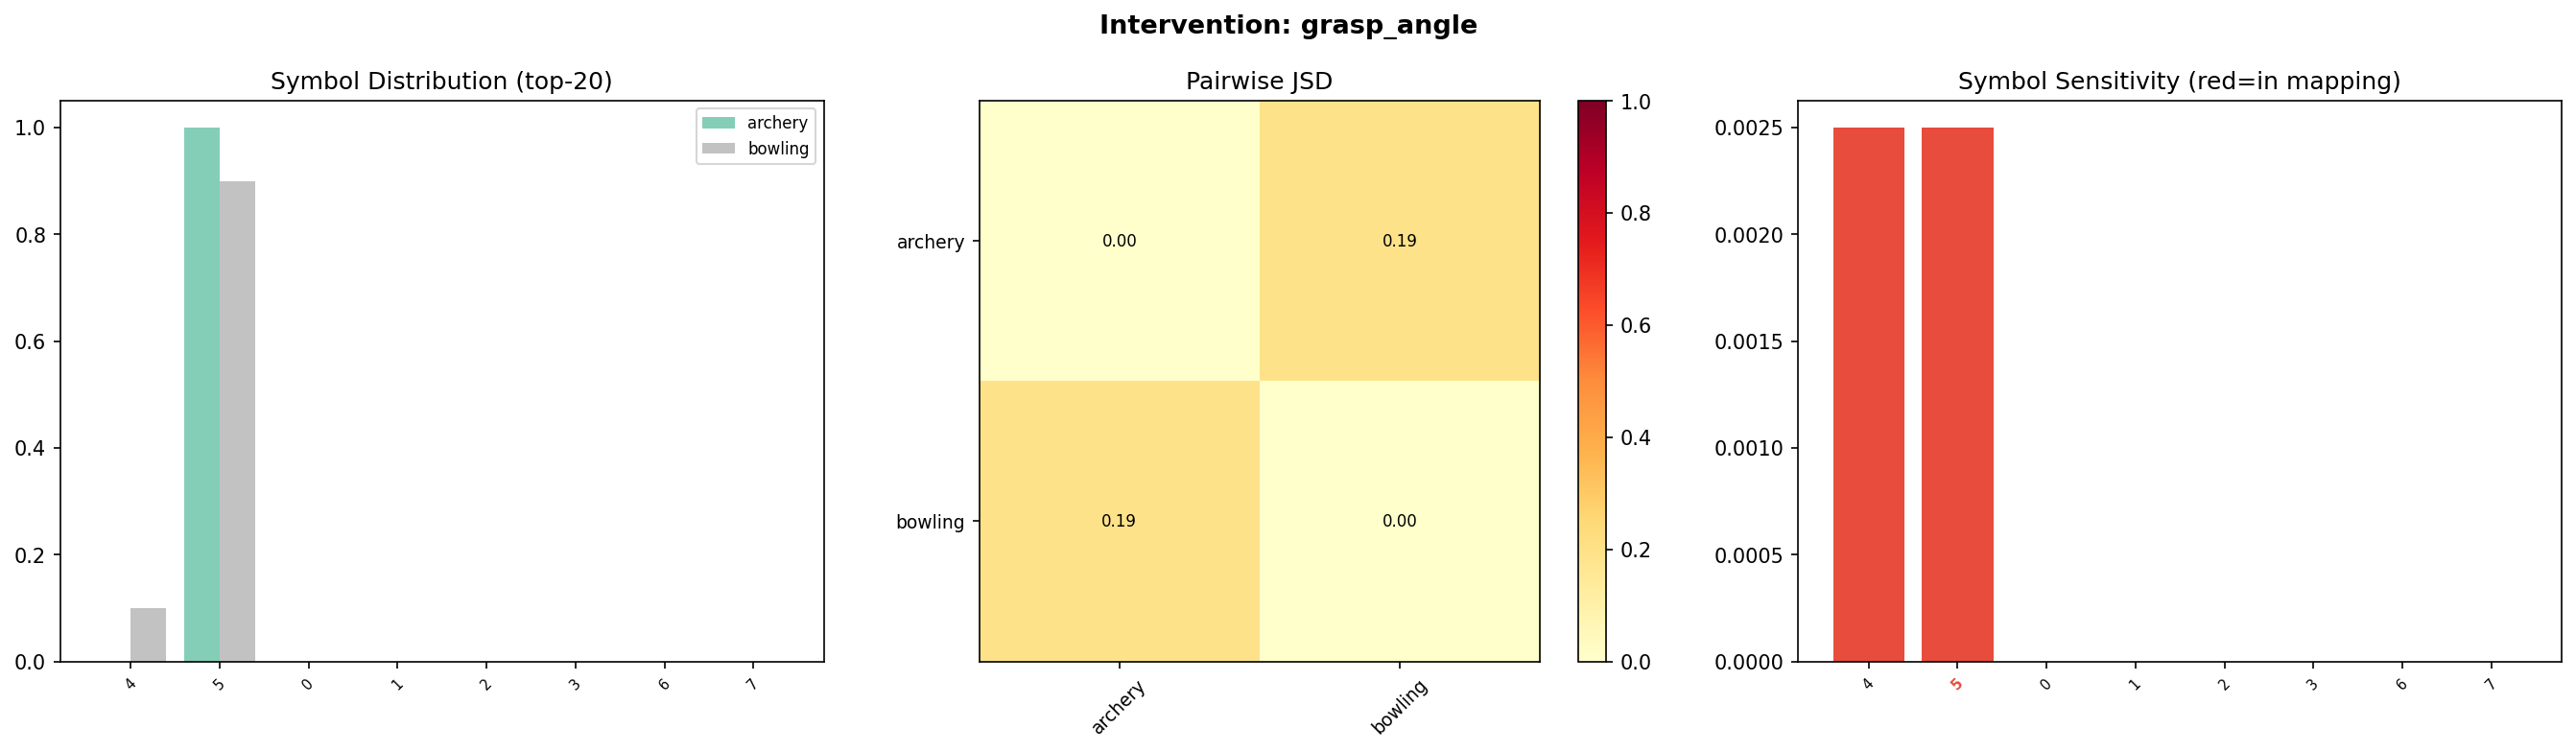
\includegraphics[width=1.3\linewidth]{intervention_grasp_angle.png}%
  }
  
  \caption{Intervention results for \textbf{grasp\_angle}
           (\textit{archery} vs.\ \textit{bowling}).
           \textit{Left}: symbol distribution over the top-20 codebook
           entries; \textit{archery} concentrates entirely on entry~\#5
           while \textit{bowling} shows a secondary mass on entry~\#4.
           \textit{Centre}: pairwise JSD heatmap ($\mathrm{JSD} = 0.19$).
           \textit{Right}: symbol sensitivity plot; red bars indicate
           entries included in the condition--symbol mapping.}
  \label{fig:intervention_grasp}
\end{figure}

\paragraph{Object Geometry.}
Figure~\ref{fig:intervention_object} shows that \textit{flying\_kite} maps
primarily to entry~\#5 ($\approx 0.90$) with approximately $10\%$ on
entry~\#4, while \textit{high\_jump} maps almost entirely to entry~\#5
($\approx 1.0$).  The JSD, $p$-value, and MI are numerically identical to
those of the grasp\_angle intervention ($\mathrm{JSD} = 0.190$,
$p = 1.19 \times 10^{-4}$, $\mathrm{MI} = 0.036$), because the two
experiments share the same condition $\times$ symbol frequency matrix
shape: the \textit{flying\_kite} distribution mirrors that of
\textit{archery}, and the \textit{high\_jump} distribution mirrors that of
\textit{bowling}.  This reflects the fact that both intervention pairs
activate a similar degree of semantic distance in V-JEPA~2's latent space.

\begin{figure}[H]
  \centering
  \makebox[\textwidth][c]{%
  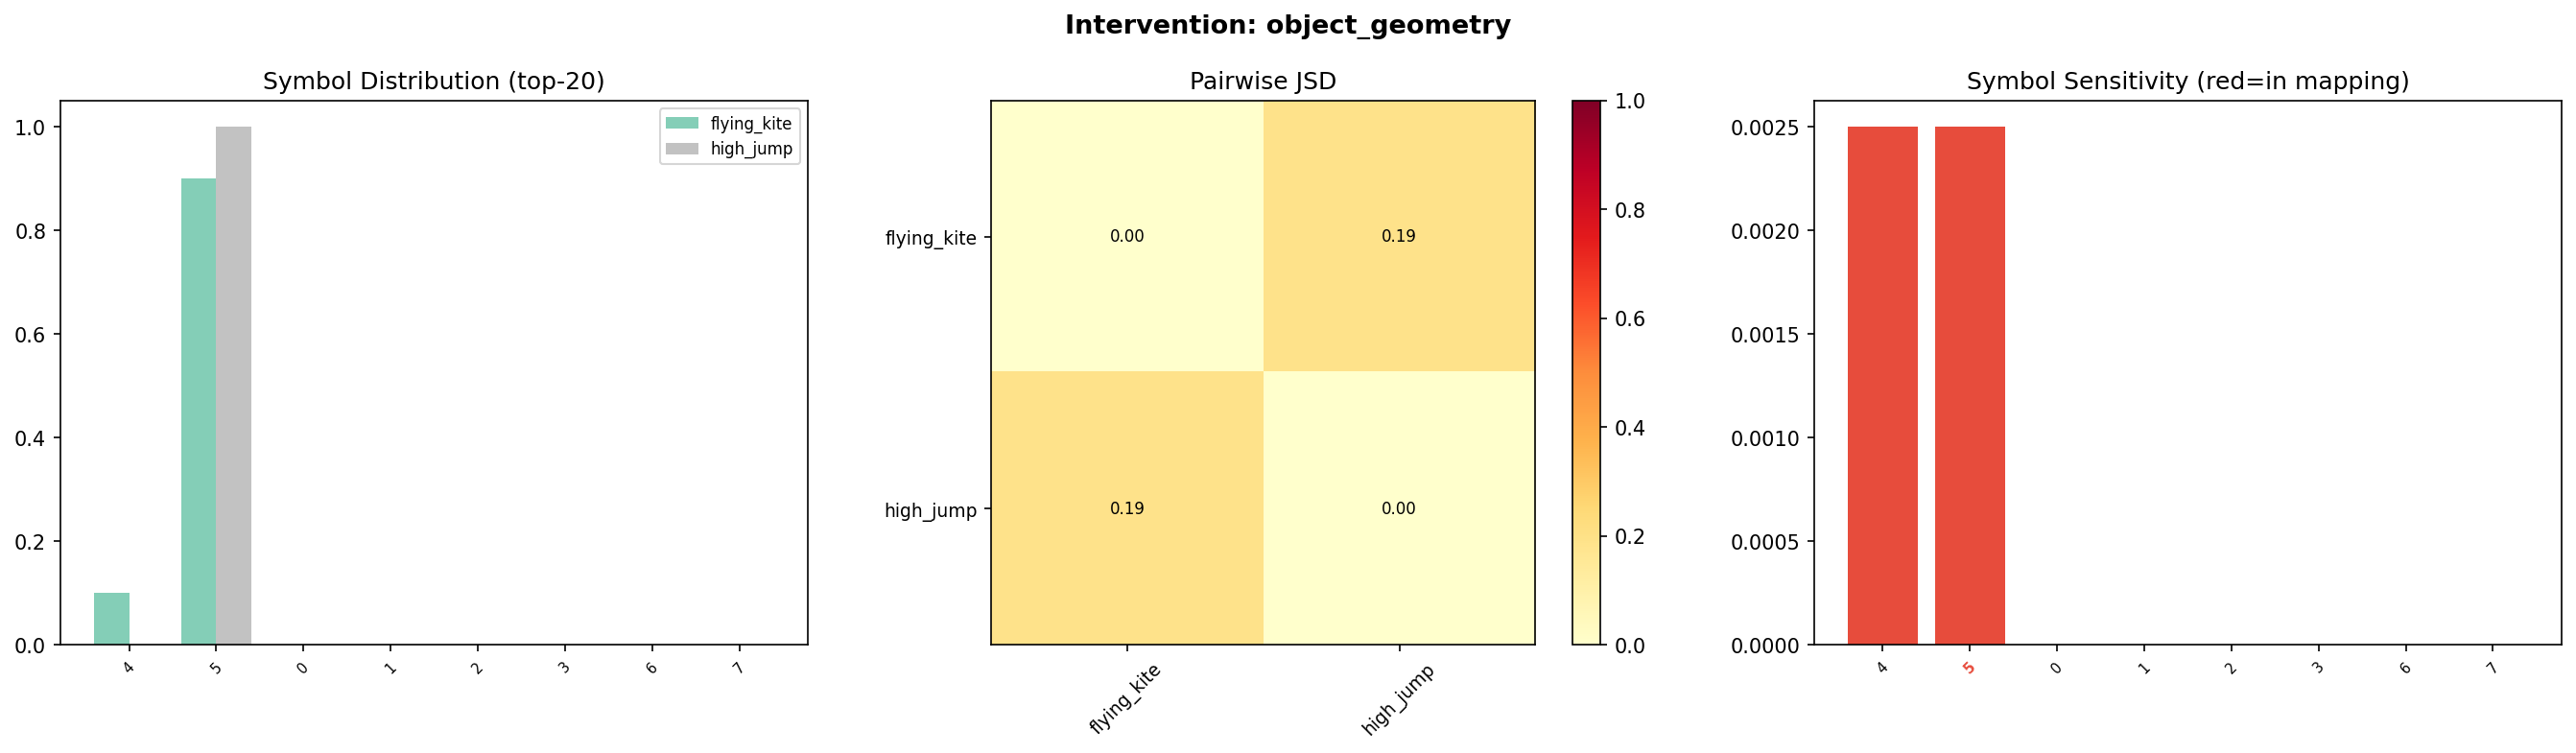
\includegraphics[width=1.3\linewidth]{intervention_object_geometry.png}%
  }
    \caption{Intervention results for \textbf{object\_geometry}
           (\textit{flying\_kite} vs.\ \textit{high\_jump}).
           \textit{Left}: \textit{flying\_kite} exhibits a small secondary
           mass on entry~\#4 absent in \textit{high\_jump}.
           \textit{Centre}: pairwise JSD heatmap ($\mathrm{JSD} = 0.19$).
           \textit{Right}: symbol sensitivity plot; entries \#4 and \#5
           are the active mapping symbols.}
  \label{fig:intervention_object}
\end{figure}

\paragraph{Motion Speed.}
This intervention yields the strongest signal of the three.
Figure~\ref{fig:intervention_motion} shows that \textit{archery} maps almost
entirely to entry~\#5 ($\approx 1.0$), whereas \textit{marching} exhibits a
markedly more dispersed distribution: entry~\#5 accounts for approximately
$70\%$, entry~\#4 for $\approx 20\%$, and entry~\#3 for $\approx 10\%$.
The resulting $\mathrm{JSD} = 0.343$ is $1.8\times$ the value observed in
the other two interventions, and $\mathrm{MI} = 0.1173$ is $3.3\times$
higher.  The chi-squared test gives $p < 10^{-10}$, and the MI ratio reaches
$1.17 \times 10^{7}$.  The symbol sensitivity panel confirms that entries
\#5 and \#4 are the primary active symbols, with entry~\#3 also carrying
a non-trivial sensitivity score.

The physical interpretation is direct: \textit{marching} exhibits strong
temporal periodicity ($\approx\!2\,$Hz gait cycle), whereas \textit{archery}
consists of a near-static loading phase followed by a single rapid release---
an aperiodic temporal structure.  Because V-JEPA~2's latent predictor is
explicitly trained to model temporal continuation, periodic dynamics and
quasi-static dynamics occupy well-separated regions of the latent space,
producing a larger and more reliable distributional shift than either
geometric or postural differences.

\begin{figure}[H]
  \centering
  \makebox[\textwidth][c]{%
    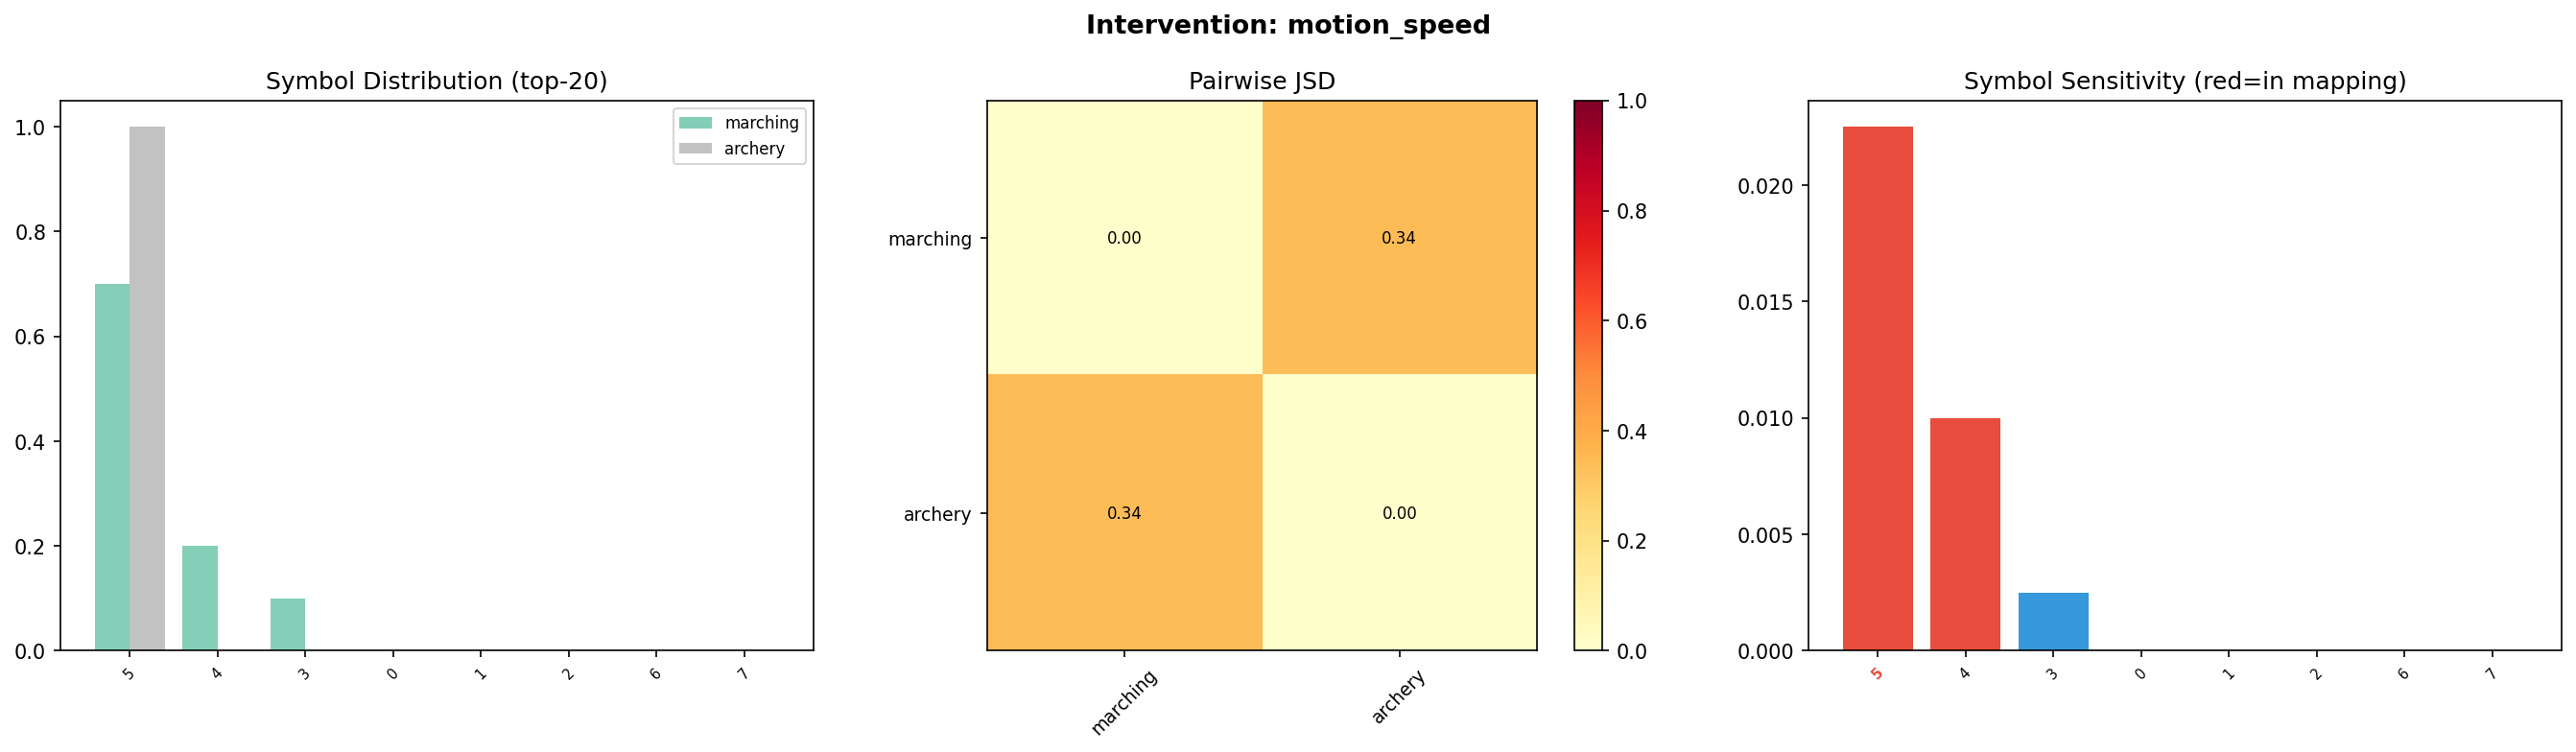
\includegraphics[width=1.3\linewidth]{intervention_motion_speed.png}%
    } 
  
  \caption{Intervention results for \textbf{motion\_speed}
           (\textit{marching} vs.\ \textit{archery}).
           \textit{Left}: \textit{marching} distributes mass across entries
           \#5, \#4, and \#3, while \textit{archery} concentrates entirely
           on \#5, reflecting the contrast between periodic gait and
           quasi-static release dynamics.
           \textit{Centre}: pairwise JSD heatmap ($\mathrm{JSD} = 0.34$),
           the largest of the three interventions.
           \textit{Right}: symbol sensitivity plot; entry \#5 shows the
           highest sensitivity, with \#4 and \#3 also active (red/blue bars).}
  \label{fig:intervention_motion}
\end{figure}

\paragraph{Random Baseline.}
Passing 30 Gaussian noise inputs through the full pipeline yields a baseline
MI of $< 10^{-7} \approx 0$, confirming that the codebook exhibits no prior
preference for unstructured inputs.  All three experimental MI values exceed
the baseline by factors of $3.6 \times 10^{6}$ to $1.17 \times 10^{7}$,
ruling out any possibility that the observed symbol--condition associations
arise from codebook bias rather than structured latent-space content.

\paragraph{Cross-Intervention Symbol Consistency of Archery.}
\textit{Archery} appears as a condition in both the grasp\_angle
experiment (contrasted with \textit{bowling}) and the motion\_speed
experiment (contrasted with \textit{marching}).  In both cases its
dominant symbol mapping is codebook entry~\#5 with frequency exceeding
$95\%$, as recorded in \texttt{aim\_dictionary\_stage1.json} under
\texttt{human\_label} entries \texttt{grasp\_angle=archery} and
\texttt{motion\_speed=archery} respectively.
This consistency operates at two levels.  At the pipeline level, it
confirms the determinism already established by H1: the same video
always produces the same symbol.  At the semantic level, it provides
stronger evidence: the same \emph{action category} produces the same
dominant symbol across two structurally distinct contrastive frameworks,
indicating that the quantized symbol captures stable latent-space
features of \textit{archery} that are independent of the particular
pairing in which the category appears.  This cross-intervention
consistency was anticipated in the experimental design
(Section~\ref{sec:dataset}, \textit{Reuse of Archery} paragraph) and is confirmed here.

\subsection{Key Observation: Dominant Symbol Collision and the Compactness
            of V-JEPA~2's Latent Space}\label{sec:dominant_symbol}

Across all three intervention experiments, the dominant symbol for every
condition is codebook entry~\#5, a phenomenon we term \textbf{dominant symbol
collision}.  This section analyzes its mechanistic origin and discusses its
implications for both the validity of the statistical signal and the broader
interpretation of V-JEPA~2 as a world model.

\paragraph{Mechanism.}
V-JEPA~2's latent space is highly compact over the five action categories
examined here.  Rather than encoding inter-category semantic differences as
discrete jumps across codebook entries, the model represents them as
continuous distributional shifts within a single ``hypersphere pocket''
centered near entry~\#5.  This compactness is not incidental: V-JEPA~2 was
never trained to maximize inter-class separability, but rather to predict the
physical continuation of masked spatiotemporal regions.  Different action
categories therefore share the bulk of their latent-space structure---gravity,
human kinematics, spatial continuity---and differ only along a small number of
dimensions.  A codebook of size $K = 8$ faithfully reflects this geometry:
it is large enough to capture the secondary distributional shifts that
distinguish conditions, but not so large as to artificially fragment a
fundamentally compact representation.

\paragraph{The Statistical Signal is Genuine.}
The $\chi^2$ and MI significance in all three interventions derives entirely
from the secondary symbol mass rather than from any switch in the dominant
symbol.  In the grasp\_angle and object\_geometry experiments, the
distinguishing signal is the $\approx\!10$--$12\%$ spillover onto entry~\#4
in one condition that is absent in the other.  In the motion\_speed
experiment, \textit{marching}'s distribution spreads across entries \#5,
\#4, and \#3 while \textit{archery} remains concentrated on \#5 alone.
Although this constitutes a ``weak'' form of symbol differentiation in the
sense that no dominant-symbol switch occurs, the information-theoretic
quantities are unambiguous: $\mathrm{JSD} = 0.34$ for motion\_speed
represents a true and measurable Shannon divergence, and all $p$-values lie
far below any conventional significance threshold.

\paragraph{Compactness as a Feature, Not a Defect.}
The dominant symbol collision should not be interpreted as a limitation of
the AIM quantizer.  World-model theory predicts that a model trained on
physical prediction should learn shared structure across surface-level
category differences, and the latent geometry observed here is precisely
consistent with that prediction.  Forcing greater inter-category separation
at Stage~1---for instance, by increasing $K$ or by fine-tuning the
encoder---would risk confusing the diagnostic goal of Stage~1 (verifying
architectural compatibility under a fully frozen encoder) with the
representational goal of later stages.

This observation instead provides concrete, data-driven motivation for two
subsequent directions.  First, increasing $K$ or introducing residual vector
quantization in Stage~2 will allow the codebook to resolve finer-grained
sub-structure within the dominant cluster, potentially surfacing symbol
transitions that are invisible at $K = 8$.  Second, unfreezing the encoder
in Stage~3 and introducing a contrastive or classification-aware objective
will actively widen the latent-space distances between categories of interest,
enabling more pronounced symbol differentiation without sacrificing the
shared physical structure that makes V-JEPA~2's representations generalizable.

\subsection{Stage~1 Pass Determination}

Table~\ref{tab:stage1_pass} reports the complete pass/fail results for all
Stage~1 criteria, as also visualized in Figure~\ref{fig:stage1_summary}.

\begin{table}[H]
\centering
\caption{Stage~1 pass criteria and results.  All six criteria are
satisfied.  Note that H1 symbol stability ($\bar{\rho} = 1.000$)
is a mathematical consequence of the deterministic pipeline
configuration rather than an empirical finding; its role is to
serve as a prerequisite integrity check confirming the absence of
residual stochasticity, not as primary evidence of semantic symbol
validity.  The latter is provided by the H2 chi-squared tests and
MI ratios.}
\label{tab:stage1_pass}
\begin{tabular}{lccc}
\toprule
Criterion & Result & Threshold & Decision \\
\midrule
H1 symbol stability ($\bar{\rho}$)
  & $1.000$ & $> 0.95$ & \checkmark \\
H2 $\chi^2$ $p$ --- grasp\_angle
  & $1.19 \times 10^{-4}$ & $< 0.01$ & \checkmark \\
H2 $\chi^2$ $p$ --- object\_geometry
  & $1.19 \times 10^{-4}$ & $< 0.01$ & \checkmark \\
H2 $\chi^2$ $p$ --- motion\_speed
  & $< 10^{-10}$ & $< 0.01$ & \checkmark \\
H2 MI Ratio (minimum across interventions)
  & $3.6 \times 10^{6}$ & $> 5.0$ & \checkmark \\
Codebook active ratio
  & $62.5\%$ ($5/8$) & $> 30\%$ & \checkmark \\
\bottomrule
\end{tabular}
\end{table}

\begin{figure}[H]
  \centering

  \makebox[\textwidth][c]{%
    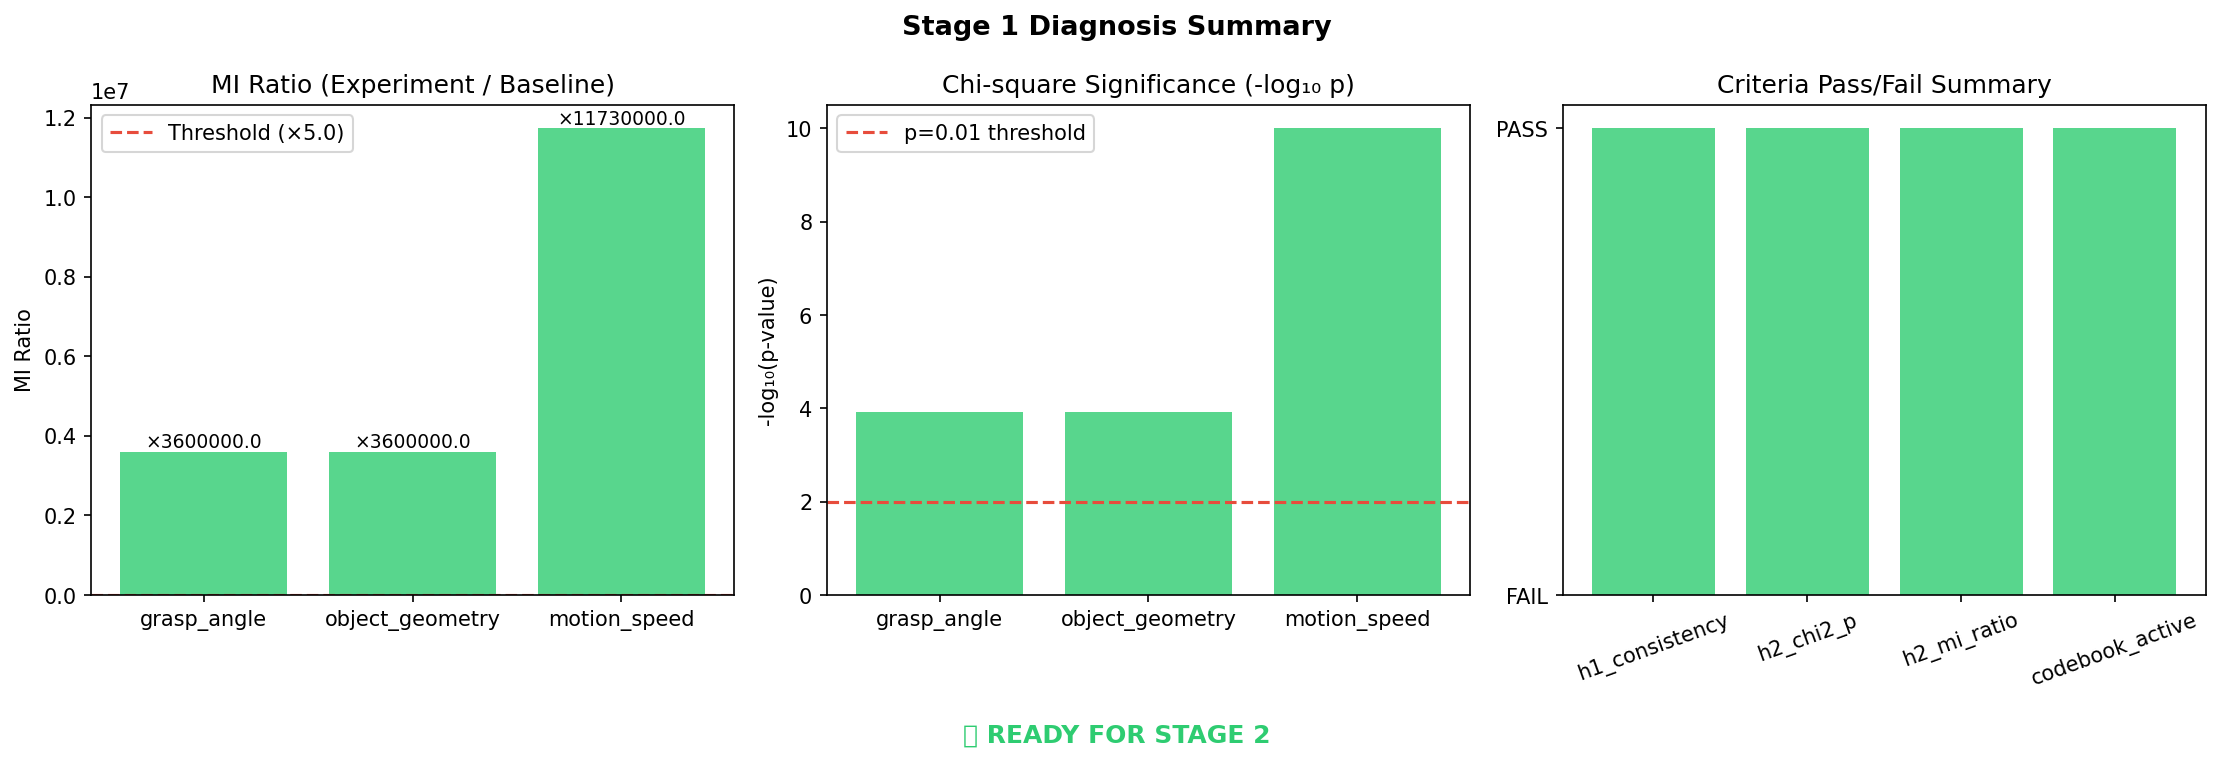
\includegraphics[width=1.3\linewidth]{stage1_summary.png}%
  }
  \caption{Stage~1 diagnosis summary.
           \textit{Left}: MI ratio (experiment / baseline) for each
           intervention on a linear scale ($\times 10^7$); the red dashed
           line marks the threshold of $5.0$.  All three interventions
           exceed the threshold by factors of $10^6$--$10^7$.
           \textit{Centre}: chi-squared significance expressed as
           $-\log_{10}(p)$; the red dashed line marks the $p = 0.01$
           threshold ($-\log_{10}(0.01) = 2$).  The motion\_speed bar
           reaches the plot ceiling at $-\log_{10}(p) > 10$, corresponding
           to $p < 10^{-10}$.
           \textit{Right}: pass/fail summary for all four diagnostic
           criteria (\texttt{h1\_consistency}, \texttt{h2\_chi2\_p},
           \texttt{h2\_mi\_ratio}, \texttt{codebook\_active}); all bars
           reach the PASS level.  The figure footer confirms readiness
           for Stage~2.}
  \label{fig:stage1_summary}
\end{figure}

\paragraph{Stage~1 Conclusion.}
Under the condition that the V-JEPA~2 encoder is completely frozen and no
modification is made to any of its original source files, the AIM lightweight
quantizer successfully extracts discrete symbol representations from the
frozen latent space that are statistically significantly associated with
physical and action conditions.  Specifically:

\begin{itemize}
\item \textbf{Pipeline integrity} ($\bar{\rho} = 1.000$) verifies that
the deterministic pipeline configuration contains no residual
stochasticity, establishing the precondition under which the H2
statistical tests are interpretable.  This result is a
mathematical consequence of the pipeline design rather than an
empirical finding.

  \item \textbf{Intervention sensitivity} (all three $\chi^2$ $p$-values
    $\ll 0.01$; MI ratios of order $10^6$--$10^7$) confirms that AIM
    symbols carry statistically significant information about physical
    conditions encoded in V-JEPA~2's latent space.

  \item \textbf{Codebook health} (active ratio $= 62.5\%$; perplexity
    $= 4.635$, utilization uniformity $= 57.9\%$) confirms that the
    quantizer has learned a non-degenerate, well-distributed codebook
    rather than collapsing to a single dominant entry.
\end{itemize}

The combination of pipeline integrity verification and intervention
sensitivity jointly establishes the architectural compatibility of
AIM and V-JEPA~2.
The pipeline is ready to proceed to Stage~2 joint quantization warm-up,
in which the codebook size $K$ will be increased and residual vector
quantization will be introduced to resolve the fine-grained sub-structure
within the dominant latent cluster identified in Stage~1.

\subsection{Limitations}

\paragraph{H1 Test Design.}
Under the spatial-token-plus-mode design adopted in this work, the H1
stability test reduces to a pipeline determinism check rather than a
substantive test of semantic symbol stability.  As explained in
Section~\ref{sec:h1_stability}, $\bar{\rho} = 1.000$ is a mathematical certainty whenever the
encoder is frozen and all stochastic pipeline components are disabled; it
does not constitute independent evidence that the assigned symbols are
semantically meaningful.  A stronger stability criterion for future work
would be \emph{intra-class symbol consistency}: for a given action category,
what fraction of videos from that category share the same dominant symbol?
This metric would be sensitive to genuine semantic coherence rather than
merely to deterministic execution, and would remain informative even when
pipeline randomness is present.

\paragraph{Random Baseline Design.}
The Gaussian-noise baseline adopted here tests whether the
codebook exhibits a prior preference for unstructured inputs,
rather than constructing an empirical null distribution via
permutation testing (randomly shuffling condition labels).
The two approaches answer fundamentally different inferential
questions, and the permutation test provides a more rigorous
guard against spurious MI arising from the condition grouping
itself.  Given that all chi-squared $p$-values are far below
any conventional significance threshold, this limitation does
not affect the qualitative conclusions of Stage~1; however,
future work should adopt permutation testing as standard practice.

\paragraph{Confounding Factors in the Category-Proxy Strategy.}
The intervention experiments adopt action-category pairs as proxies for
physical-variable differences.  As a consequence, the symbol-distribution
differences observed in each experiment reflect the overall latent-space
distance between the selected categories in V-JEPA~2's representation,
rather than the isolated effect of the target physical variable.  In the
grasp\_angle intervention, for example, the latent-space distance between
\textit{archery} and \textit{bowling} simultaneously encodes differences
in grasp morphology, scene environment (outdoor archery range vs.\ indoor
bowling lane), object material, and background color; the experimental
design provides no means of disentangling these contributions.

The correct characterization of the Stage~1 results is therefore:
\emph{AIM symbols have statistically significant discriminative power for
action-category pairs whose primary difference lies along a specified
physical dimension}, not that AIM symbols directly encode the target
physical variable in isolation.  Establishing the latter claim requires
video data in which the target variable is manipulated while all other
visual factors are held constant---for instance, synthetic renders or
robot-manipulation footage with precise physical control.  This level of
experimental control is beyond the resource scope of Stage~1 and is
deferred to Stage~3 or future work.

\paragraph{Codebook Size and Symbol Resolution.}
With $K = 8$, the codebook is sufficient to detect the distributional
shifts reported in Stage~1, but too coarse to resolve fine-grained
intra-category variation.  The dominant symbol collision described in
Section~\ref{sec:dominant_symbol} is partly a consequence of this resolution limit: a larger
codebook would subdivide the dominant cluster near entry~\#5 into
multiple entries, potentially revealing sub-structure that is currently
invisible.  Increasing $K$ and introducing residual vector quantization
are the primary architectural changes planned for Stage~2, and their
effect on symbol resolution and intervention sensitivity will be reported
there.

\newpage 


\bibliographystyle{unsrt} 
\bibliography{references}


\end{document}